\documentclass{article}

\title{Computer Systems and Architecture - Notes}
\author{Harvey Hyatt}
\date{}

\usepackage[a4paper, total={7in, 10in}]{geometry}
%\usepackage{graphicx}
%\graphicspath{ {images/} }

\begin{document}
\maketitle

\section{The von Neumann Architecture}
Even in a simple program, the computer needs to be able to perform many different tasks:
\begin{itemize}
\item Arithmetic
\item Logic
\item Program flow
\item Comparisons
\item Input/Output
\item Store internal state of program
\end{itemize}

\paragraph{Instructions and Data} Computer programs are made up of Instructions (usually a sequential set) and Data to be manipulated by the instructions.
\vspace{1mm}
Both of these are represented (physically) in the same way - you can not tell them apart without looking at them in detail. Because of this we need to store instructions and data in separate regions of memory, and have separate ``datapaths'' for instructions and data.

\paragraph{Requirements of a Computing Device}
\begin{itemize}
\item Load the program from some external device
\item Process instructions in the correct order (need mechanism to keep track of progress)
\item Access data in accordance with program's instructions
\item Perform computations
\item Take decisions according to computation results
\item Send results of computations to external device
\end{itemize}

\paragraph{The CPU in Context}
%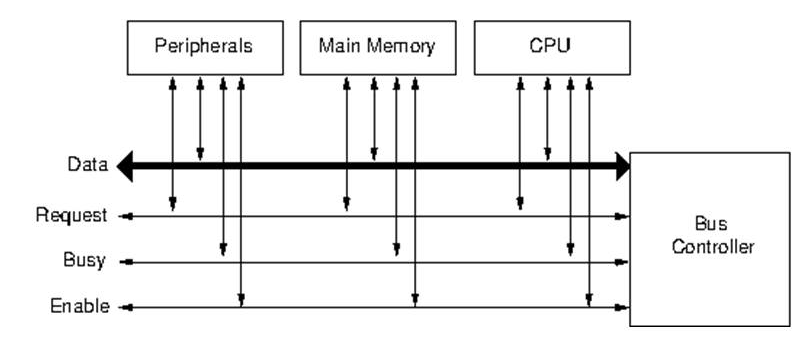
\includegraphics[width=\linewidth]{csa1.png}
Bus allows for communication between CPU, Main Memory and Peripherals
Data, Request, Busy and Enable lines

Load/store unit: knows how to talk to the bus and request access
Knows what to do with data or instructions recieved

Requests to obtain data from outside world come from Program Counter and

Program Counter keeps track of where you are in the program
Counts memory addresses of instructions
Only stores \textit{locations} of instructions
Requests instruction at address from load/store unit
Instruction stored in Instruction Register

Control Unit knows what to do with an instruction (has a lookup table)
Takes input from Instruction Register
Can tell load/store unit to get specific data

Data from outside world stored in Registers
Each register stores one item of data

ALU (Arithmetic-Logic Unit) does calculations - recieves data and stores result in registers

\paragraph{Executing Programs}
Fetch-Decode-Execute Cycle:
Load - get the program and store it somewhere accessible (main memory), store address of first instruction in PC (program counter)
Fetch - Load instructions from memory into CPU (Instruction register), Update PC with address of next instruction
Decode - Determine what the instruction is supposed to do, calculate memory address of data, fetch data etc.
Execute - Perform calculation, store result, update PC if control instruction

Instruction cycle is not the same as Clock cycle:
Instruction cycle is synchronised by clock cycle
Some instructions are single-cycle, some are multi-cycle
Clock cycle triggers successive stages of the instruction cycle
Clock cycle is neccessary because circuit X may or may not complete faster than circuit Y
Change from low voltage to high voltage signifies new stage of clock cycle

Case Study: MIPS R4000 - Late 80's
Similar to von Neumann but separate interfaces to instructions and data (modified harvard architecture)
Cache: larger than register
One for instructions and one for data

Intel Core: Heavily modified Harvard architecture

\end{document}
